\section{Introduction}
%\subsection{General Objectives for building an autonomous sailboat}
This paper introduces the autonomous sailboat \textsc{Avalon} as seen in figure
\ref{fig:avalon}. The general objective for building an autonomous sailing
vessel is to further research and development in the area of unmanned,
autonomous robotic vehicles that are exposed to heavy environmental conditions
such as the Atlantic Ocean. It has been established that there is a demand for
autonomous sailboats to be used for ocean sampling and surveillance
\cite{cruz:ase} but also for the implementation of this type of software in
manned sailing vessels. Either by passively proposing optimal sailing routes or
by actively supporting the sailor in dangerous situations by piloting the sail
or rudders, an integrated autonomous sailing system could back up and
facilitate a lot of situations. For example, if a single hand sailor falls over
board, the system could detect this incident and automatically execute a Man
Over Board manoeuvre.

\subsection{Our Goals and Objectives for this Work}
Our boat \textsc{Avalon} was designed to compete in the \textsc{Microtransat}
Challenge and thus has to withstand the harsh conditions on the Atlantic Ocean.

The goal of this paper is to present a software that is
capable of calculating the optimal path to reach a given destination as quickly
as possible, and the design of a controller able to safely and efficiently
guide the sailboat along the calculated path, taking into account the current
environmental conditions, such as wind speed.
\hide{Furthermore, it should be able to respond to a possible shortness of
energy by adjusting the control parameters or changing the mode of sailing.}


\subsection{Review of Existing Autonomous Sailing Boats}
An autonomous sailboat has to be capable of sailing without human intervention.
That means, that all tasks that are normally carried out by the sailor on a
conventional sailboat have to be done autonomously. That involves navigation
as well as working the rudder and sail in order to steer the defined course.
Other autonomous sailboats have been developed mostly by \textsc{Microtransat}
participants \cite{briere2008iar}, \cite{stelzer2008}, \cite{alves:fas},
\cite{sauze2008dcs}, but also commercially usable products \cite{harborwing}
have been built. In contrast to most of the existing work, we use a path
planner to avoid obstacles. Additionally, our controller switches between many
different modes of sailing, in order to make better use of wind shifts.

\section{A Boat Designed for Survival}
To provide an insight into the platform that was used to implement the proposed
software, this section summarises some details about the main components of
{\sc Avalon}. The mechanical system was more comprehensively described in
\cite{giger2009}. Table \ref{tab:avalon_data} shows the major technical details
of {\sc Avalon}.
\begin{figure}[b!]
\centering
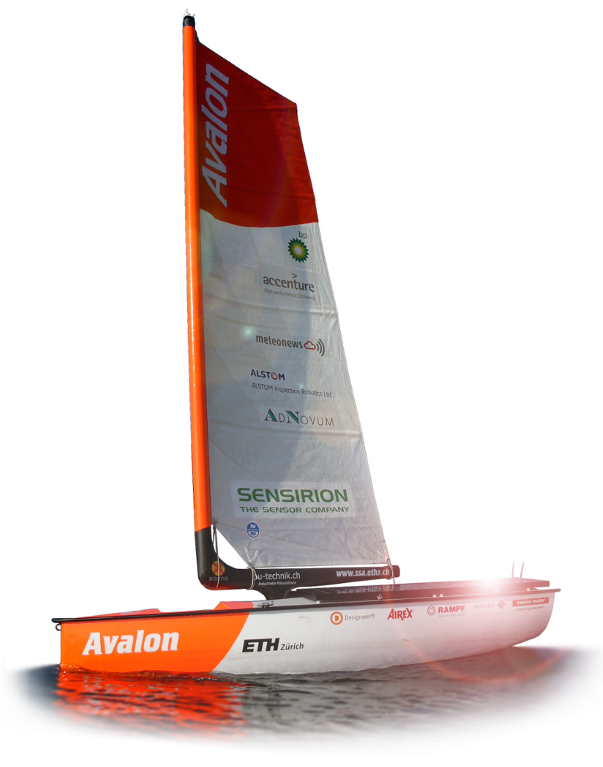
\includegraphics[height=0.8\columnwidth]{pics/avalon.png}
\caption{Avalon ready to sail on the lake of Z\"urich}
\label{fig:avalon}
\end{figure}

\subsection{Rig}
The rigging system is one of the most important parts of the whole
assembly. A defect in its structure will inevitably cause the whole project to
fail. The following aspects were considered for the design:
\begin{itemize}
\item High loads and forces on the mechanical structures due to
strong winds and heavy weather conditions.
\item Highest demands on reliability. There is no chance to
repair anything throughout the journey.
\item Preferably efficient force transmission from the actuator to the sail in order to save as much energy as
possible
\end{itemize}

During the design phase it turned out that a balanced rig prevails over a
conventional rig.
\hide{
The balanced rig is much more efficient regarding energy
consumption than any other conventional rig. The force needed to position the
sail is reduced by over 50\% due to the balanced distribution of
the sail load. Furthermore, }\textsc{Avalon}'s rig does not use any ropes
that could generate knots and jams. It is pivoted on a central
bearing without shrouds and stays. The result is a simple and reliable construction.
%
\subsection{Hull}
\hide{The hull design is based on form parameters, e.g. length, draft and
beam. Parameters were used as input data for B-spline curves and
surfaces. Instead of modifying those curves and surfaces, we used
constrained optimisation algorithms to generate the geometry. The algorithm
minimises a target function, which is defined so that a certain combination of
parameters results in a desired hull shape.}

The hull was designed using the CAE software \textsc{FRIENDSHIP-Framework} and
was laminated inside a female mold using glass fibre
sandwich. Epoxide resin was sucked into dry glass fibre material by
vacuum in a so called \textit{Infusion Process}. Compared to
conventional laminating, this method is much cleaner and more
convenient.

%---------------------------------------------------------
%basicdata: AVALON
%---------------------------------------------------------
\begin{table}[htb]

    \begin{center}
     \caption{Technical Data of \textsc{Avalon}}
	\label{tab:avalon_data}
%        \begin{tabular}[h!]{p{0.15\textwidth}| p{0.2\textwidth}| p{0.05\textwidth}}
        \begin{tabular}[htb]{l|l|l}
            \hline
            \emph{Variable}    &   \emph{Description} &   \emph{Value}\\ \hline\hline
            $L_{OA}$    &   Length over all	& $3.95\,m$\\
            $B_{max}$   &   Maximal beam	& $0.7\,m$\\
            $T$         &   Draft without keel  & $0.25\,m$\\
            $D_{max}$	&   Draft over all	& $2\,m$\\
            $H_{rigg}$	&   Height of the rigg  & $5.7\,m$\\
            $A_{sail}$	&   Total sail area     & $8.4\,m^2$\\
            $\nabla$    &   Submerged volume    & $0.44\,m^3$\\
            \hline
        \end{tabular}
    \end{center}
\end{table}


\begin{figure}[htb]
\centering
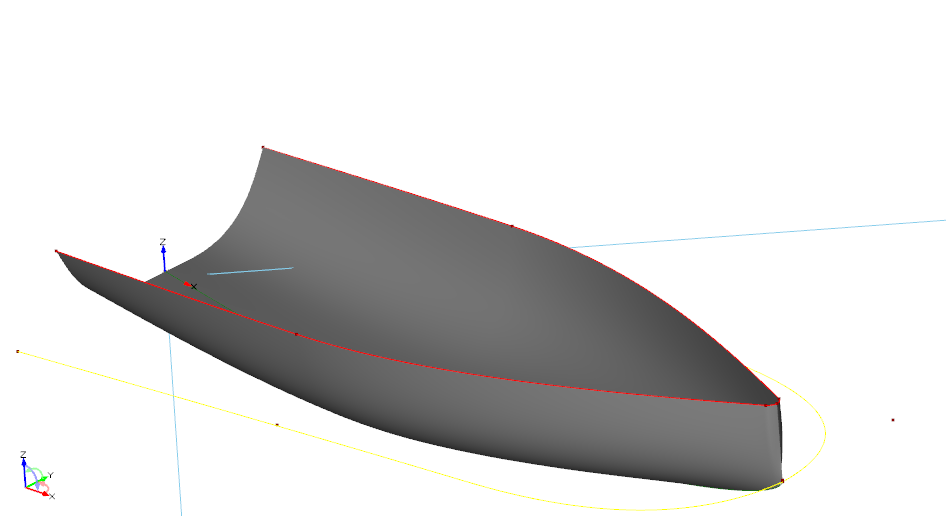
\includegraphics[width=0.37\textwidth]{pics/hull.png}
\caption{Hull} \label{fig:hull}
\end{figure}

%
\subsection{Keel and Rudder}
\subsubsection{Keel}
In order to achieve a sufficient righting moment and stability
during heavy weather situations, {\sc Avalon}'s keel with a draft of
two meters consists of a slim fin with a 160\,kg ballast bulb.

The fin and parts of the bulb were made of high-modulus carbon fibre
in precisely milled polyurethane female molds. After hardening and
tempering, the bulb was filled with lead and the two halves were
glued together.

\begin{figure}[htb]
\centering
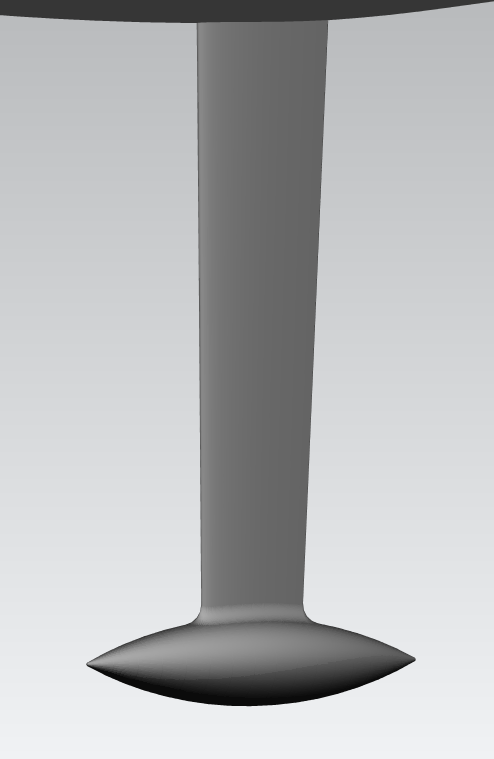
\includegraphics[width=2.7cm]{pics/keel.png}\hfill
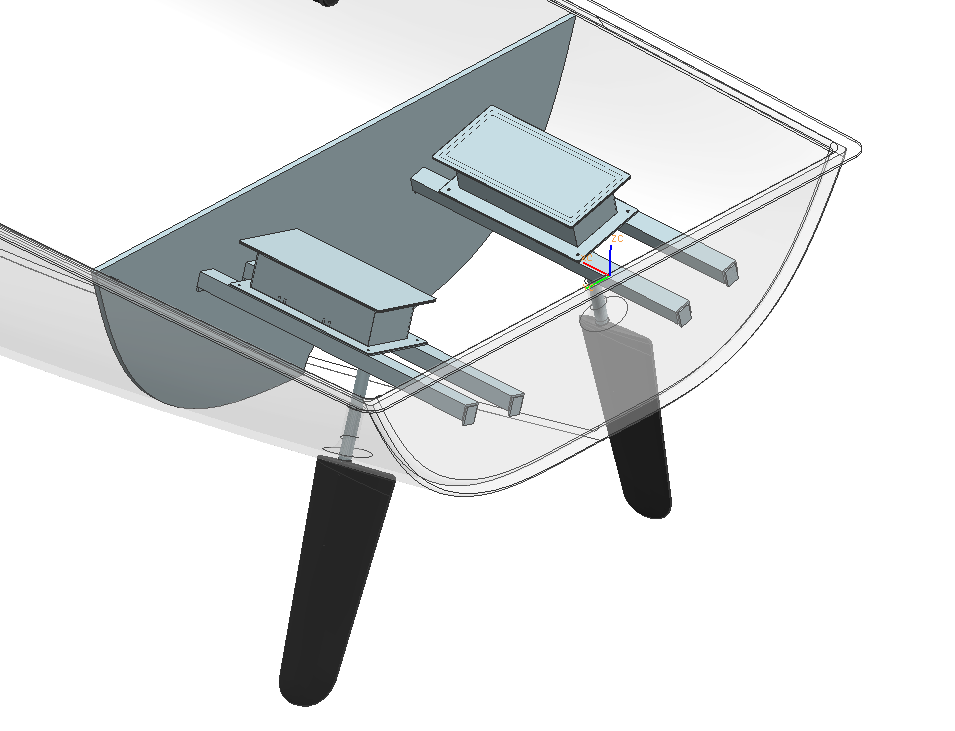
\includegraphics[width=4.5cm]{pics/rudder.png}
% \caption{Twin rudder system} \label{fig:cadrudder}
\caption{Keel with fin and ballast bulb (left), Twin rudder system (right)} \label{fig:cadkeel}
\end{figure}

\subsubsection{Rudder}
A twin-rudder system was selected for {\sc Avalon} to make sure to
have sufficient steering effect in every sailing situation. Angular
mounted twin-rudders provide better control at high
heeling angles compared to single rudders.

Assembled inside the hull, the rudder actuators are well sealed and
protected against water and humidity.

% \begin{figure}[htb]
% \centering
% 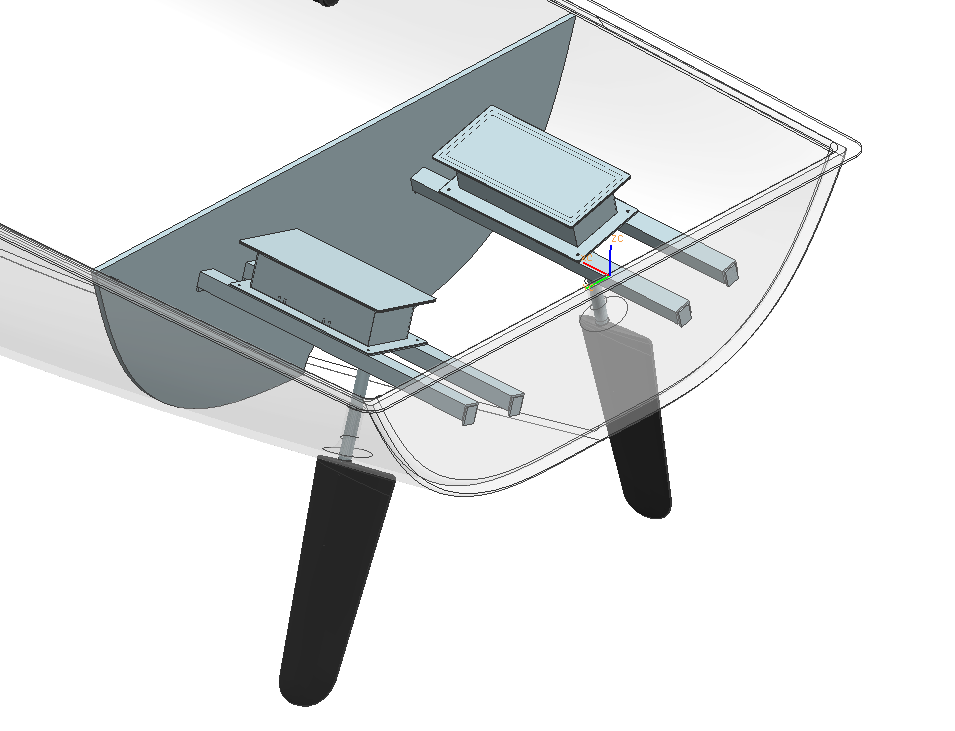
\includegraphics[width=4cm]{pics/rudder.png}
% \caption{Twin rudder system} \label{fig:cadrudder}
% \end{figure}
%
\subsection{Power Supply}
The main power supply is realised through two square meters of solar panels providing
a total of 360\,Wp. The collected energy is stored in four lithium-manganese
batteries. Each battery consists of 70 single cells and has a capacity of
600\,Wh at a nominal voltage of 25.2\,volts. Lithium-manganese batteries were
chosen mainly because of their weight but also because they are fairly safe to
use.

For back-up power, the boat has a direct-methanol fuel cell on
board. This fuel cell is automatically activated when the voltage
drops under a certain value, the \emph{switch on} voltage. It then
charges the batteries until the \emph{switch off} voltage is
reached. In theory, the solar cells provide enough power for the
boat's systems. The fuel cell only serves in case of enduring bad
weather  or other unforeseeable circumstances.


